\documentclass[12pt,utf8]{beamer}
\usetheme{Frankfurt}
\usecolortheme{default}
\setbeamercovered{transparent}

%Wichtige Standard Pakete!
\usepackage[ngerman]{babel}
\usepackage{xcolor}
\usepackage{graphicx}

%------------------------------------------------------------
%This block of code defines the information to appear in the
%Title page
\title[LSN zur zeitnahen Detektion von Wasserschäden]{Luftfeuchtigkeits-Sensor-Netzwerk zur zeitnahen Detektion von Wasserschäden auf Basis von LoRa(WAN)}
%\subtitle{subtitle}
\author{Sidney Göhler \\ Ilja Buschujew}
\institute[HTW Berlin]{Projekt Netzbasierte Systeme\\
Informations- und Kommunikationstechnik (M. Eng.)\\
Hochschule für Technik und Wirtschaft Berlin}
\date[ProNeSy WS 21/22] % (optional)
{11. Februar 2022}

%End of title page configuration block
%------------------------------------------------------------

% %------------------------------------------------------------
% %The next block of commands puts the table of contents at the 
% %beginning of each section and highlights the current section:
% 
% \AtBeginSection[]
% {
%   \begin{frame}
%     \frametitle{Gliederung}
%     \tableofcontents[currentsection]
%   \end{frame}
% }
% 
% %------------------------------------------------------------

\begin{document}
%The next statement creates the title page.
\frame{\titlepage}
%---------------------------------------------------------
%This block of code is for the table of contents after
%the title page
\begin{frame}
\frametitle{Gliederung}
\tableofcontents
\end{frame}

%---------------------------------------------------------

\section{Einleitung}
\begin{frame}
\frametitle{Einleitung}
\begin{itemize}
 \item Problem: Schimmliger Keller
 \item Idee: Sensornetzwerk nach dem Urban-Common Prinzip
 \item Ziel: Werteorientierte Gesellschaft mit mehr Selbstbestimmung
\end{itemize}

\end{frame}

\section{Vorstellung der Projektidee}
\begin{frame}
\frametitle{Vorstellung der Projektidee}
\begin{itemize}
 \item Erstellung einer Plattform zum Sammeln und ggf. Teilen von eigenen Sensorwerten mit anderen
 \item Einsatzmöglichkeiten:
 \begin{itemize}
  \item Frühwarnsystem
  \item Beweismittel bei Sachschaden
 \end{itemize}
\end{itemize}

\end{frame}

\subsection{Prinzip des Urban-Commons}
\begin{frame}
\frametitle{Prinzip des Urban-Commons}
\begin{itemize}
\item „Kooperative Möglichkeit, die vernachlässigten Bedürfnisse zu befriedigen und den eigenen physischen und sozialen Lebensraum selbst zu gestalten“ \footnote{https://www.boell.de/de/2015/05/26/urban-commons}
\item Offene communitybasierte Initiativen:
\begin{columns}
% \centering

\column{0.35\textwidth}
\begin{figure}

\includegraphics[scale=0.2]{bilder/ttn}
\end{figure}

\column{0.3\textwidth}
\begin{figure}

\includegraphics[scale=0.2]{bilder/luftdaten}
\end{figure}

\column{0.3\textwidth}
\begin{figure}
 
\includegraphics[scale=0.2]{bilder/freifunk}
\end{figure}
\end{columns}

% \begin{itemize}
% \item freifunk.net
% \item thethingsnetwork.org
% \item luftdaten.info
% \end{itemize}
\end{itemize}
\end{frame}

\section{Hardware}
\begin{frame}
\frametitle{Hardware}
\begin{itemize}
\item Verwendete Hardware:
\begin{itemize}
 \item 2 Pycom-Mikrocontroller mit LoRa Modul
 \item 2 Antennen
 \item 1 DHT11/DHT22 Sensor
\end{itemize}
\begin{columns}
 \column{0.4\textwidth}
\begin{figure}
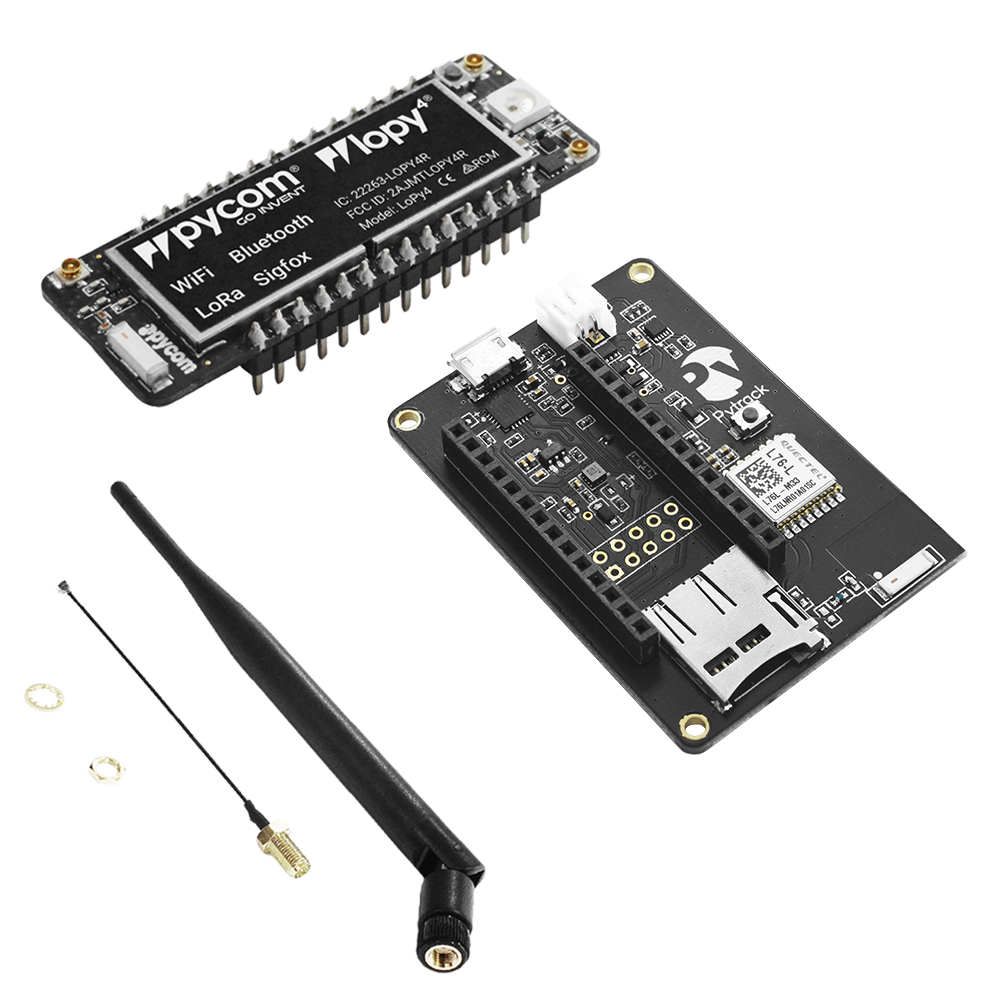
\includegraphics[scale=0.1]{bilder/hardware}
\end{figure}
\column{0.5\textwidth}
\begin{figure}
 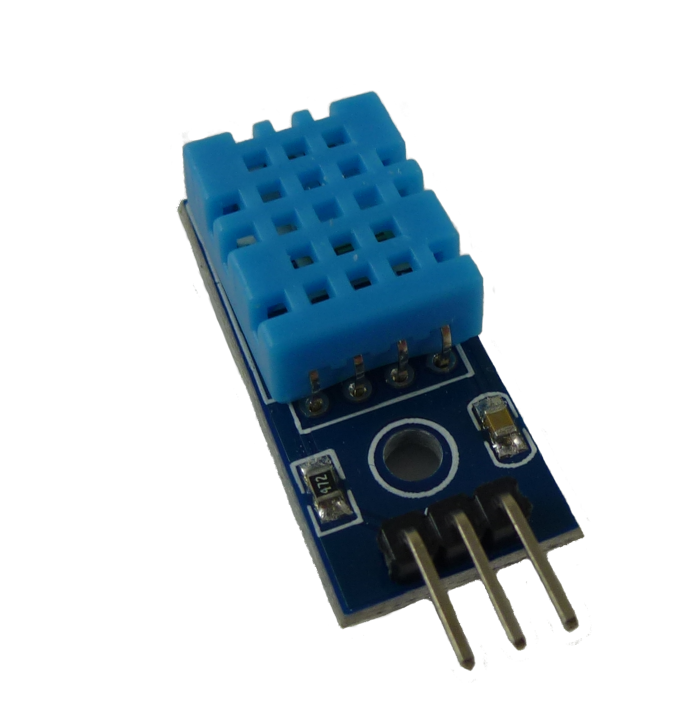
\includegraphics[scale=0.25]{bilder/dht11}
\end{figure}
\end{columns}
\end{itemize}
\end{frame}

\subsection{Blockdiagramm LoPy4}
\begin{frame}
\frametitle{Blockdiagramm LoPy4}
\begin{figure}
 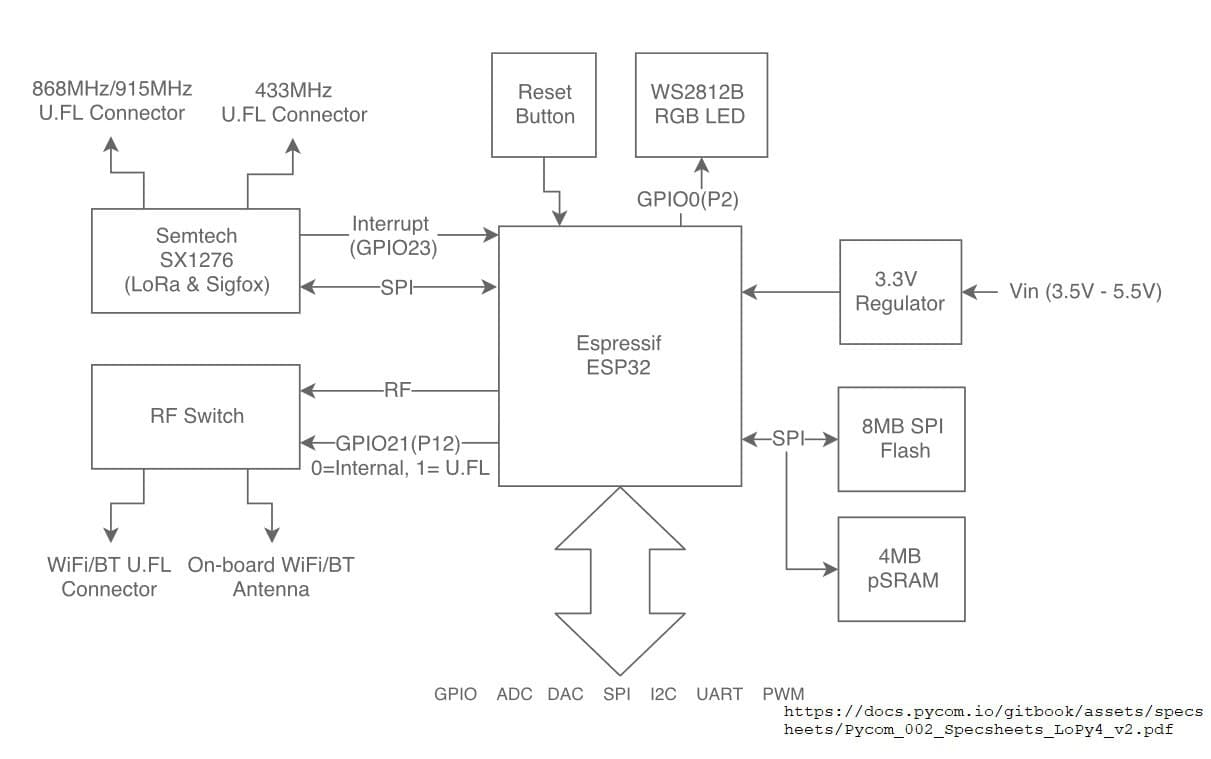
\includegraphics[scale=0.3]{bilder/blockdiagram_lopy}
\end{figure}
\end{frame}

\subsection{Schaltplan}
\begin{frame}
\frametitle{Schaltplan}
\begin{figure}
 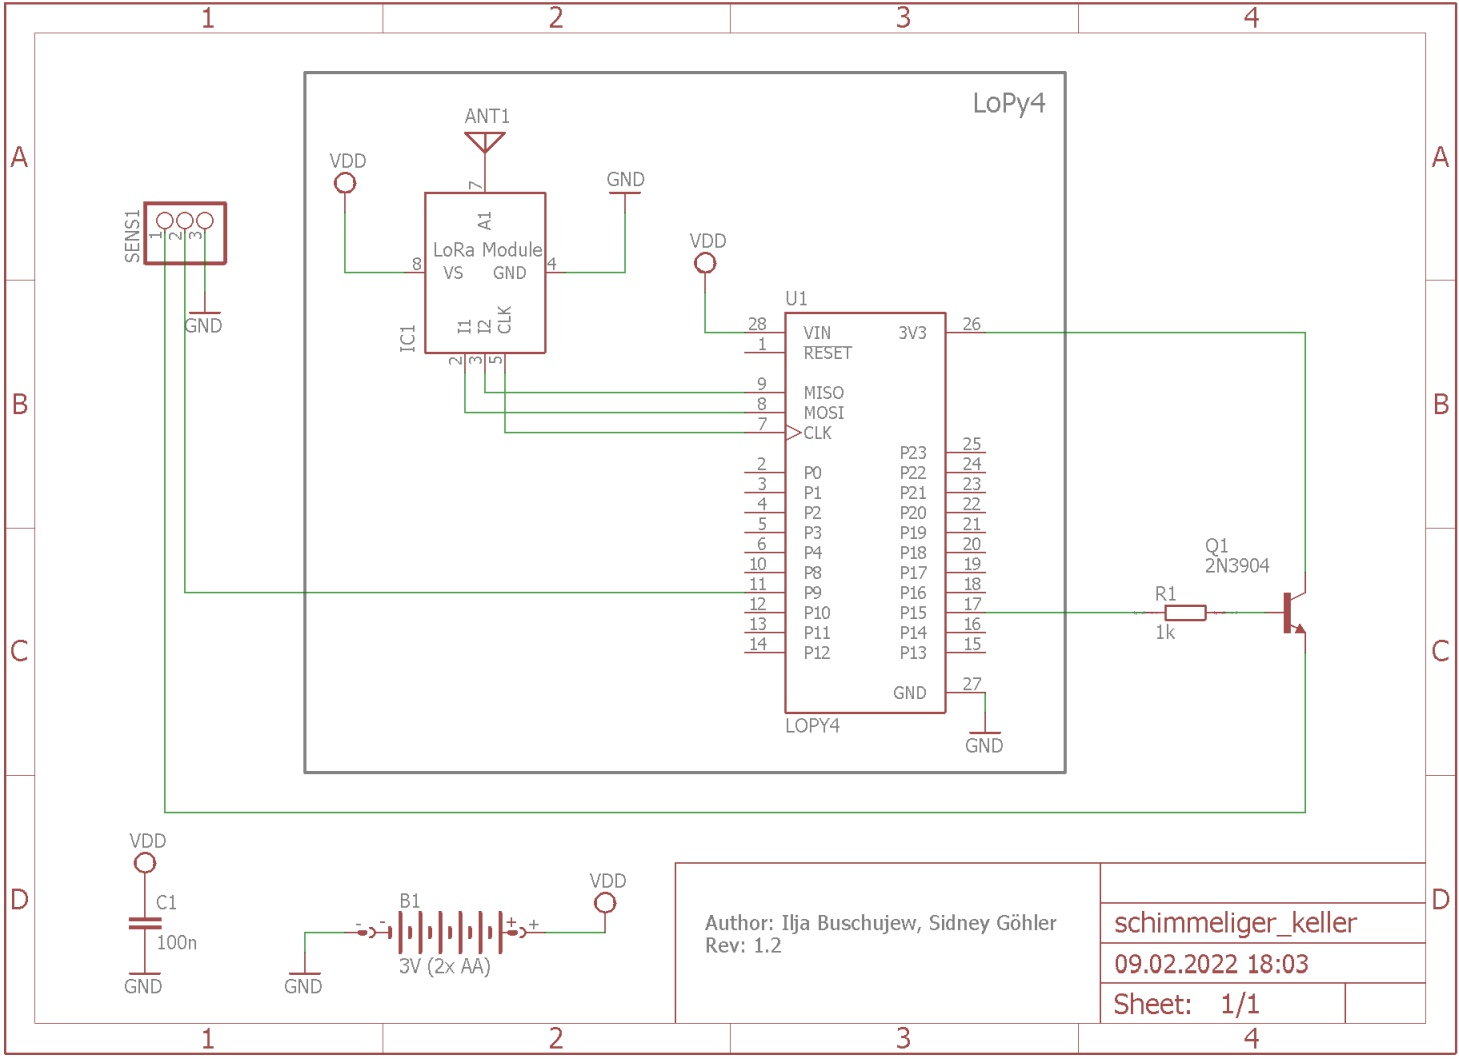
\includegraphics[scale=0.2]{bilder/LoRaSender_Schaltung}
\end{figure}
\end{frame}

\section{Software}
\subsection{Blockschaltbild}
\begin{frame}
\frametitle{Software: Blockschaltbild}
\begin{itemize}
\item Programmiersprache: MicroPython/Python 
\end{itemize}
\begin{figure}
 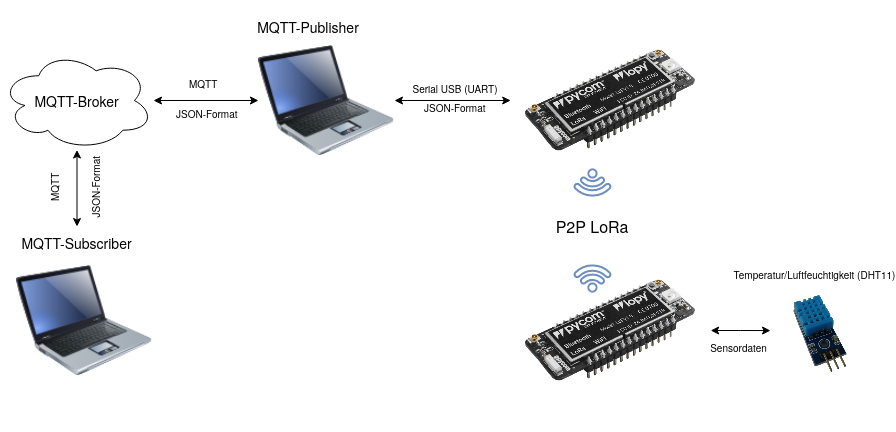
\includegraphics[scale=0.35]{bilder/Blockschaltbild_ProNeSy}
\end{figure}

\end{frame}

\subsection{DHT11 Datenübertragung}
\begin{frame}
\frametitle{Software: DHT11 Datenübertragung}
\begin{itemize}
\item Serielle Schnittstelle (Single-Wire Two-Way)
\end{itemize}
\begin{figure}
 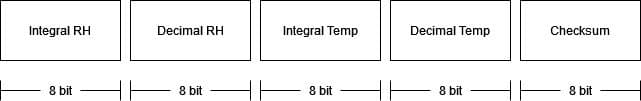
\includegraphics[scale=0.5]{bilder/dht11_dataframe}
\end{figure}
\begin{figure}
 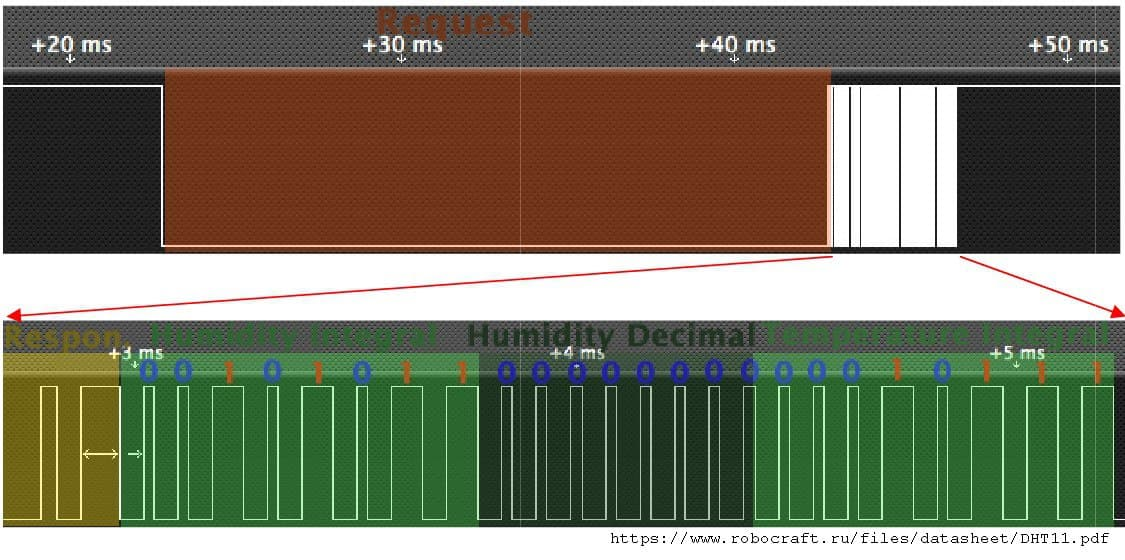
\includegraphics[scale=0.3]{bilder/dht11_pegel}
\end{figure}
\end{frame}

\subsection{LoRa}
\begin{frame}
\frametitle{Software: LoRa}
\begin{itemize}
\item Leitungsloses Übertragungsverfahren auf der Bitübertragungsschicht
\item Chirp-Spread-Spectrum-Modulationstechnik

\end{itemize}
\begin{figure}
 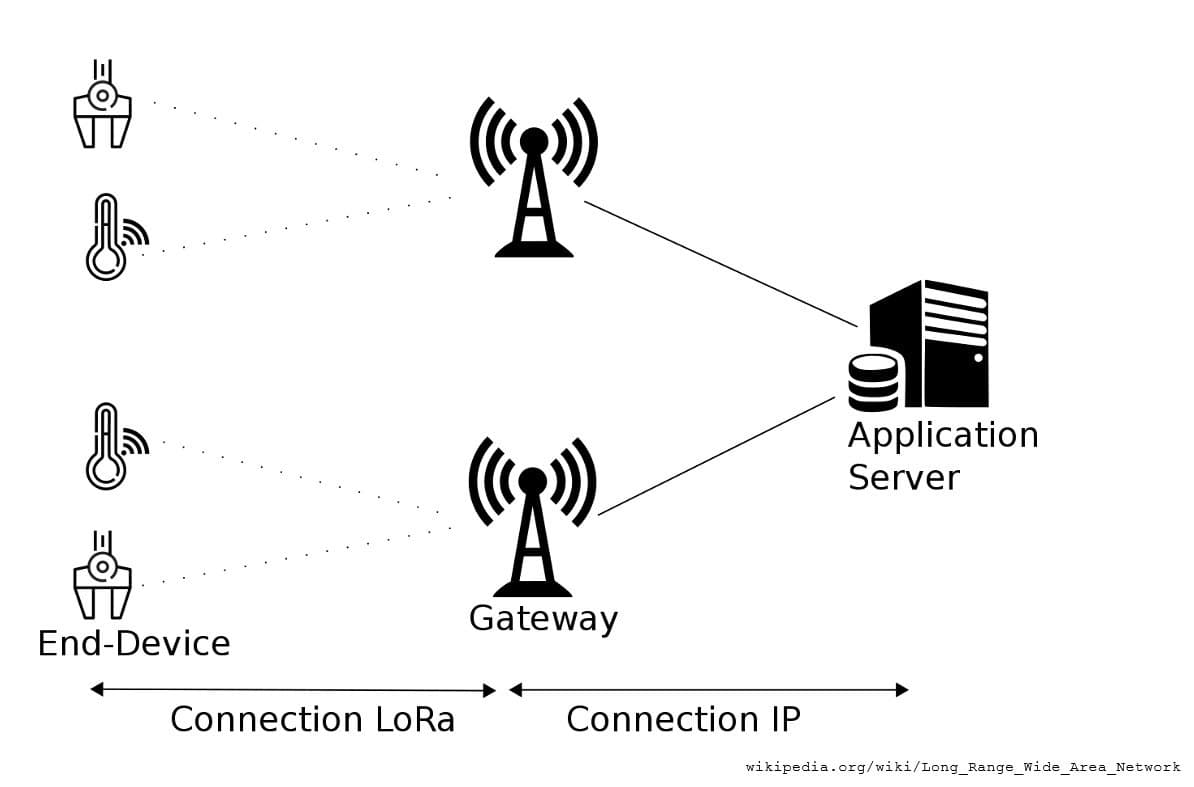
\includegraphics[scale=0.2]{bilder/LoRaWAN}
\end{figure}
\end{frame}

\section{Vorführung}
\begin{frame}
\frametitle{Vorführung}
\begin{itemize}
\item Dashboard MQTT topics (Adafruit IO):
\begin{itemize}
 \item \textbf{Temperatur:} io.adafruit.com/b\_ilja/feeds/temperature
 \item \textbf{Luftfeuchtigkeit:} io.adafruit.com/b\_ilja/feeds/humidity
 \item \textbf{Alarm-Temp:} io.adafruit.com/b\_ilja/feeds/alarm-temp
 \item \textbf{Alarm-Hum:} io.adafruit.com/b\_ilja/feeds/alarm-hum
\end{itemize}
\end{itemize}
\end{frame}

\section{Simulation Batterielaufzeit}
\begin{frame}
\frametitle{Simulation Batterielaufzeit}
\begin{figure}
 
\includegraphics[scale=0.5]{bilder/jupyter}
\end{figure}
\end{frame}

\section{Ausblick}
\begin{frame}
\frametitle{Ausblick}
\begin{itemize}
\item Erweiterung von LoRa-LoRa zu LoRaWAN
\item Benutzung von mehreren Sensorknoten an einem LoRa-Gateway
\item Erweiterung der Software zur Einbindung von mehreren Sensorkomponenten
\item Batteriebetrieb in Hardware umsetzen
\item Alternative MQTT-Broker evaluieren
\item Alternative Dashboard Möglichkeiten 
\end{itemize}
\end{frame}

\section{Quellen}
\begin{frame}
\frametitle{Quellen}
\begin{itemize}
\item robocraft.ru/files/datasheet/DHT11.pdf
\item github.com/JurassicPork/DHT\_PyCom/tree/pulses\_get
\item pycom.io/product/lopy4/
\item lora-wan.de/
\item io.adafruit.com/
\item uni.de/redaktion/urban-commons
\item boell.de/de/2015/05/26/urban-commons
\item wikipedia.org/wiki/Long\_Range\_Wide\_Area\_Network
\end{itemize}
\end{frame}


\end{document}
